\section{二次规划与锥规划}
\label{sec:opt-con-quadratic-conic}

前三节的结论对一般的$f,g_i,h_j$成立。设计算法时，还要知道目标和约束具体是什么形状：同一个问题，写成二次规划、二阶锥规划还是半正定规划，决定了可以调用哪种子问题求解器、需要多少存储。本节按“目标与约束能写成什么结构”辨认三类常用模型，并说明哪些问题可以等价改写进来。这三类模型彼此包含：线性规划是二次规划的特例，凸二次规划可以写成二阶锥规划，二阶锥约束又可以写成半正定约束；它们不是互斥的分类，而是表达能力逐级增强、求解代价逐级增加的一组工具。为避免与最小二乘的数据矩阵$\bm A,\bm b$混淆，本节把线性约束写成$\bm E\bm x=\bm e$与$\bm G\bm x\leq\bm r$。

\subsection{二次规划}
\label{sec:opt-con-qp}

\paragraph{定义与凸性}
在线性约束下最小化平方误差，是最常见的约束问题之一。例如要求系数非负的最小二乘$\min\frac12\lVert\bm A\bm x-\bm b\rVert_2^2$、$\bm x\geq\bm0$，展开后目标是$\frac12\bm x^\top\bm A^\top\bm A\bm x-\bm b^\top\bm A\bm x+\text{常数}$。一般地，称
\begin{equation}
\label{eq:opt-con-qp}
  \min_{\bm x}\ \frac12\bm x^\top\bm P\bm x+\bm a^\top\bm x
  \quad\text{s.t.}\quad\bm E\bm x=\bm e,\quad\bm G\bm x\leq\bm r
\end{equation}
为\term{二次规划}（quadratic program），其中$\bm P$对称。目标的Hessian处处等于$\bm P$，所以目标凸当且仅当$\bm P\succeq\bm0$；$\bm P$有负特征值时，问题是非凸二次规划，一般可能有许多局部最小点，求全局最优通常是困难的。预算分配例是$\bm P=\bm I$的凸二次规划。最小二乘的线性方程解法见\BookChapterRef{chap:linear-equations-and-optimization}{卷一“线性方程与矩阵方程”章}，这里关心的是约束带来的新结构。

\paragraph{三种情形中的计算职责}
没有约束时，凸二次目标的最优条件是线性方程$\bm P\bm x=-\bm a$；它有解当且仅当$\bm a$在$\bm P$的值域中。只有等式约束时，KKT条件仍是线性方程组
\[
  \begin{bmatrix}\bm P&\bm E^\top\\\bm E&\bm0\end{bmatrix}
  \begin{bmatrix}\bm x\\\bm\nu\end{bmatrix}
  =\begin{bmatrix}-\bm a\\\bm e\end{bmatrix},
\]
其系数矩阵就是式~\eqref{eq:opt-con-kkt-matrix}的KKT矩阵；$\bm E$行满秩且$\bm P$在$\ker\bm E$上正定时，引理~\ref{lem:opt-con-kkt-matrix}保证它可逆，解唯一。等式二次例就是这种情形，一次线性求解便给出$(\bm x^\star,\nu^\star)$。

含不等式时困难在于不知道哪些约束活跃。若猜中最优点的活动集$I$，把$I$中的不等式当作等式，问题就退化为等式约束二次规划；解出后检查两件事：未列入$I$的约束是否满足，列入$I$的约束乘子是否非负。两项都通过，由凸问题的KKT充分性即得最优解；否则调整猜测，加入被违反的约束或删去乘子为负的约束。这就是\term{活动集法}（active-set method）的思路。预算分配例$\tau=2$时，先猜$I=\emptyset$得$\bm x=\bm c=(2,1)^\top$，违反预算；改猜$I=\{1\}$，解出$\bm x=(3/2,1/2)^\top$、$\lambda_1=1/2\geq0$，非负约束也满足，停止。活动集的组合数随约束数指数增长，最坏情形下活动集法可能尝试很多次；内点法（第~\ref{sec:opt-con-interior-point}节）则绕开了组合选择。

\paragraph{半正定但不正定时}
$\bm P\succeq\bm0$但奇异时，目标沿$\ker\bm P$的方向是线性的。若$\bm a$在某个可行的零空间方向上有负分量，目标无下界：无约束的$\min\frac12x_1^2+x_2$沿$x_2\to-\infty$无下界。若$\bm a$与这些方向正交，最优点不唯一：$\min\frac12x_1^2$的最优解集是整条$x_2$轴。加入约束可以改变这两种情形，例如再要求$x_2\geq0$，$\min\frac12x_1^2+x_2$的唯一解变为$\bm0$。所以检查二次规划时要分别核对：$\bm P$的惯性（凸性）、零空间方向上目标与约束的关系（有界性与唯一性），以及可行域是否非空。第~\ref{sec:opt-con-sqp}节的序列二次规划在每一步求解一个二次规划，那里同样要先做这些检查。

\subsection{二阶锥规划}
\label{sec:opt-con-socp}

\paragraph{二阶锥}
许多约束形如“某个仿射向量的欧氏范数不超过一个仿射函数”，例如鲁棒线性约束或带误差球的定位问题。把这种约束抽象出来，就是下面的集合。

\begin{definition}[二阶锥与二阶锥规划]
\label{def:opt-con-socp}
集合$K_k=\{(\bm u,t)\in\mathbb R^{k-1}\times\mathbb R:\lVert\bm u\rVert_2\leq t\}$称为\term{二阶锥}（second-order cone）。形如
\[
  \min_{\bm x}\ \bm a^\top\bm x\quad\text{s.t.}\quad\lVert\bm F_i\bm x+\bm f_i\rVert_2\leq\bm c_i^\top\bm x+d_i\ (i=1,\dots,K),\quad\bm E\bm x=\bm e
\]
的问题称为\term{二阶锥规划}（second-order cone program），每条约束即$(\bm F_i\bm x+\bm f_i,\bm c_i^\top\bm x+d_i)\in K_{k_i}$。
\end{definition}

二阶锥是凸锥：范数的三角不等式与正齐次性保证它对加法和非负倍数封闭。约束的右端$\bm c_i^\top\bm x+d_i$不必另外要求非负，因为左端非负，满足约束就已迫使右端非负。图~\ref{fig:opt-con-soc}画出$k=3$时的二阶锥，它的形状像一个冰淇淋筒：高度为$t$的水平截面是半径为$t$的圆盘。点$(\bm u,t)=((0.3,0.2)^\top,0.8)$满足$\lVert\bm u\rVert_2\approx0.361\leq0.8$，位于锥内。

\begin{figure}[!htbp]
  \centering
  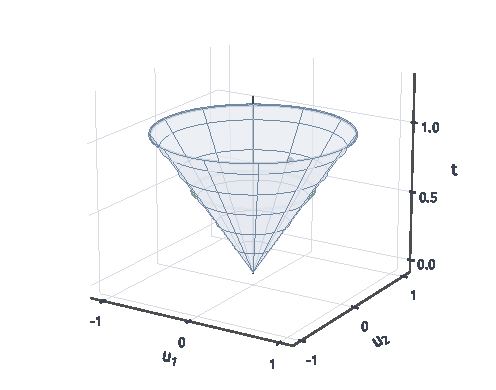
\includegraphics[width=84mm]{figures/03-optimization-evolution-and-signals/01-optimization/matplotlib/c5-soc/figure.pdf}
  \caption{$\mathbb R^3$中的二阶锥$\{(u_1,u_2,t):\sqrt{u_1^2+u_2^2}\leq t\}$，画出$0\leq t\leq1$的部分。蓝色圆为$t=1$的截面边界，绿色圆为$t=0.6$的截面边界，黑点$(0.3,0.2,0.8)$位于锥内。}
  \label{fig:opt-con-soc}
\end{figure}

\paragraph{把非线性不等式改写为锥成员条件}
改写的基本手段是引入上图变量。最小化范数$\lVert\bm A\bm x-\bm b\rVert_2$等价于在$\lVert\bm A\bm x-\bm b\rVert_2\leq t$下最小化$t$：任何可行$(\bm x,t)$都有$t\geq\lVert\bm A\bm x-\bm b\rVert_2$，最优时$t$恰取等号，所以两问题的最优值相同，最优$\bm x$也相同。平方范数需要多一步。对$s,t\geq0$，
\begin{equation}
\label{eq:opt-con-rotated-cone}
  \lVert\bm u\rVert_2^2\leq st\iff\left\lVert\begin{pmatrix}2\bm u\\s-t\end{pmatrix}\right\rVert_2\leq s+t,
\end{equation}
因为右式平方后为$4\lVert\bm u\rVert_2^2+(s-t)^2\leq(s+t)^2$，即$4\lVert\bm u\rVert_2^2\leq4st$；而右式本身已蕴含$s+t\geq|s-t|$，即$s,t\geq0$。

\paragraph{凸二次规划的锥形式}
设$\bm P\succeq\bm0$，取一个因子分解$\bm P=\bm F^\top\bm F$（如Cholesky分解或由谱分解得到）。目标$\frac12\bm x^\top\bm P\bm x+\bm a^\top\bm x=\frac12\lVert\bm F\bm x\rVert_2^2+\bm a^\top\bm x$。引入$t$，问题等价于
\[
  \min_{\bm x,t}\ t+\bm a^\top\bm x\quad\text{s.t.}\quad\left\lVert\begin{pmatrix}2\bm F\bm x\\2-t\end{pmatrix}\right\rVert_2\leq2+t,
\]
这里用式~\eqref{eq:opt-con-rotated-cone}取$\bm u=\bm F\bm x$、$s=2$，约束等价于$\frac12\lVert\bm F\bm x\rVert_2^2\leq t$。原问题的每个可行$\bm x$配上$t=\frac12\lVert\bm F\bm x\rVert_2^2$都可行且目标值不变；反过来，锥问题的任一可行$(\bm x,t)$都有$t\geq\frac12\lVert\bm F\bm x\rVert_2^2$，丢掉$t$后$\bm x$的原目标值不超过锥目标值。所以两问题最优值相等，最优$\bm x$相同，恢复时只需丢弃辅助变量。

这样的改写扩大了变量维数，还需要先对$\bm P$作分解。若$\bm P$稀疏而$\bm F$稠密，或$\bm P$只能通过矩阵向量积访问，保留二次结构直接求解往往更省；改写的好处是能把多种二次项和范数项统一交给锥规划求解器。改写也有边界：含平方项不等于凸。约束$\bm x^\top\bm Q\bm x\leq1$在$\bm Q$有负特征值时定义的是非凸集（如$x_1^2-x_2^2\leq1$是两条双曲线之间的区域），不能写成二阶锥约束；这类非凸二次约束要等到第~\ref{sec:opt-con-sdp-relaxation}节用松弛处理。

\subsection{半正定规划}
\label{sec:opt-con-sdp}

\paragraph{矩阵变量与迹内积}
有些约束天然落在矩阵上，例如协方差矩阵必须半正定、矩阵的最小特征值要尽量大。设$\mathbb S^k$为$k\times k$实对称矩阵组成的空间，在其上使用\term{Frobenius内积}（Frobenius inner product）$\langle\bm X,\bm Y\rangle=\operatorname{tr}(\bm X\bm Y)=\sum_{a,b}X_{a,b}Y_{a,b}$。线性目标与线性测量都写成这种内积。

\begin{definition}[半正定规划]
\label{def:opt-con-sdp}
给定$\bm C,\bm A_1,\dots,\bm A_m\in\mathbb S^k$与$\bm b\in\mathbb R^m$，问题
\[
  \min_{\bm X\in\mathbb S^k}\ \langle\bm C,\bm X\rangle\quad\text{s.t.}\quad\langle\bm A_i,\bm X\rangle=b_i\ (i=1,\dots,m),\quad\bm X\succeq\bm0
\]
称为（标准型）\term{半正定规划}（semidefinite program）。
\end{definition}

半正定锥$\{\bm X\succeq\bm0\}$是凸锥：若$\bm v^\top\bm X\bm v\geq0$、$\bm v^\top\bm Y\bm v\geq0$对所有$\bm v$成立，非负组合也满足。判断$\bm X\succeq\bm0$等价于全部特征值非负（\BookChapterRef{chap:linear-analysis}{卷一“谱和奇异值”章}），这与逐元素非负是两回事。$\begin{bmatrix}1&2\\2&1\end{bmatrix}$各元素为正，特征值却是$3$与$-1$；$\begin{bmatrix}1&-1\\-1&1\end{bmatrix}$有负元素，特征值$0$与$2$都非负。

图~\ref{fig:opt-con-psd-disk}把这一差别画出来。取迹为$1$的$2\times2$对称矩阵$\bm X=\begin{bmatrix}a&b\\b&1-a\end{bmatrix}$，它由两个数$(a,b)$决定。$\bm X\succeq\bm0$等价于对角元非负且行列式$a(1-a)-b^2\geq0$，即$(a-\frac12)^2+b^2\leq\frac14$：半正定的矩阵组成一个圆盘。逐元素非负要求$0\leq a\leq1$、$b\geq0$，是一条竖带的上半部分。圆盘的下半部分有负元素却半正定，竖带中圆盘以外的部分元素非负却不半正定。

\begin{figure}[!htbp]
  \centering
  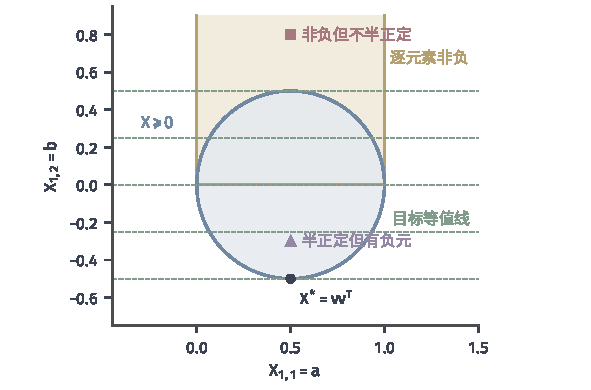
\includegraphics[width=100mm]{figures/03-optimization-evolution-and-signals/01-optimization/matplotlib/c5-psd-disk/figure.pdf}
  \caption{迹为$1$的$2\times2$对称矩阵$\begin{bmatrix}a&b\\b&1-a\end{bmatrix}$。蓝色圆盘为半正定矩阵$(a-\frac12)^2+b^2\leq\frac14$，黄色区域为逐元素非负的矩阵。红色方块$(0.5,0.8)$元素非负但不半正定，紫色三角$(0.5,-0.3)$半正定但有负元素。绿色虚线是目标$\langle\bm C,\bm X\rangle=2+2b$（$\bm C=\begin{bmatrix}2&1\\1&2\end{bmatrix}$）的等值线，最小值在圆盘最低点$\bm X^\star=\bm v\bm v^\top$处取得。}
  \label{fig:opt-con-psd-disk}
\end{figure}

\paragraph{Schur补}
半正定约束常用来表达非线性不等式，工具是Schur补。

\begin{lemma}[Schur补判别]
\label{lem:opt-con-schur}
设$\bm A\succ\bm0$，则$\begin{bmatrix}\bm A&\bm B\\\bm B^\top&\bm D\end{bmatrix}\succeq\bm0$当且仅当\term{Schur补}（Schur complement）$\bm D-\bm B^\top\bm A^{-1}\bm B\succeq\bm0$。
\end{lemma}

\begin{proof}
令$\bm T=\begin{bmatrix}\bm I&-\bm A^{-1}\bm B\\\bm0&\bm I\end{bmatrix}$，它可逆，且
\[
  \bm T^\top\begin{bmatrix}\bm A&\bm B\\\bm B^\top&\bm D\end{bmatrix}\bm T=\begin{bmatrix}\bm A&\bm0\\\bm0&\bm D-\bm B^\top\bm A^{-1}\bm B\end{bmatrix}.
\]
合同变换保持半正定性，块对角矩阵半正定当且仅当两块都半正定，而$\bm A\succ\bm0$已知。
\end{proof}

例如$\lVert\bm x\rVert_2^2\leq t$等价于$\begin{bmatrix}\bm I&\bm x\\\bm x^\top&t\end{bmatrix}\succeq\bm0$：这里$\bm A=\bm I$，Schur补为$t-\bm x^\top\bm x$。非线性的平方约束变成了对$(\bm x,t)$线性的矩阵不等式。引理要求左上块正定；左上块只半正定时，还需要“$\bm B$的列在$\bm A$的值域中”这一类附加条件，并把逆换成伪逆，不能直接套用上面的结论。

\paragraph{对偶锥与矩阵乘子}
半正定规划的对偶要用矩阵形式的乘子。对锥$K$，称$K^*=\{\bm Y:\langle\bm Y,\bm X\rangle\geq0\ \text{对所有}\ \bm X\in K\}$为它的\term{对偶锥}（dual cone）。非负象限的对偶锥仍是非负象限，这正是标量不等式乘子要求非负的原因。半正定锥也是自对偶的：若$\bm X,\bm Y\succeq\bm0$，则$\langle\bm Y,\bm X\rangle=\operatorname{tr}(\bm Y^{1/2}\bm X\bm Y^{1/2})\geq0$；反之若$\langle\bm Y,\bm X\rangle\geq0$对全部$\bm X\succeq\bm0$成立，取$\bm X=\bm v\bm v^\top$得$\bm v^\top\bm Y\bm v\geq0$。

对标准型半正定规划，把约束$\bm X\succeq\bm0$的乘子取为$\bm S\succeq\bm0$，Lagrange函数为$\langle\bm C,\bm X\rangle-\sum_iy_i(\langle\bm A_i,\bm X\rangle-b_i)-\langle\bm S,\bm X\rangle$，关于$\bm X$的下确界有限当且仅当$\bm C-\sum_iy_i\bm A_i=\bm S$。于是对偶问题为
\[
  \max_{\bm y}\ \bm b^\top\bm y\quad\text{s.t.}\quad\bm S=\bm C-\sum_iy_i\bm A_i\succeq\bm0.
\]
弱对偶可以直接核对：原始可行$\bm X$与对偶可行$\bm y$满足$\langle\bm C,\bm X\rangle-\bm b^\top\bm y=\langle\bm S,\bm X\rangle\geq0$。乘子的“非负”在这里是矩阵半正定$\bm S\succeq\bm0$，而不是逐元素非负。零间隙时$\langle\bm S,\bm X\rangle=0$，对两个半正定矩阵这等价于$\bm S\bm X=\bm0$，是矩阵形式的互补松弛。与标量情形一样，强对偶需要正则条件：若原问题有正定的可行矩阵$\bm X\succ\bm0$且最优值有限，则零间隙成立且对偶最优值达到\scite{math-boyd2004convex}。

\begin{example}[最小特征值的半正定规划]
\label{ex:opt-con-sdp-eigen}
取$\bm C=\begin{bmatrix}2&1\\1&2\end{bmatrix}$，最小化$\langle\bm C,\bm X\rangle$，约束$\operatorname{tr}\bm X=1$、$\bm X\succeq\bm0$。在图~\ref{fig:opt-con-psd-disk}的坐标中，目标为$2a+2b+2(1-a)=2+2b$，在圆盘最低点$(a,b)=(\frac12,-\frac12)$取最小值$1$，此时$\bm X^\star=\bm v\bm v^\top$，$\bm v=(1,-1)^\top/\sqrt2$。对偶问题为$\max y$、$\bm C-y\bm I\succeq\bm0$，即$y\leq\lambda_{\min}(\bm C)=1$，对偶最优值也是$1$。乘子矩阵$\bm S=\bm C-\bm I=\begin{bmatrix}1&1\\1&1\end{bmatrix}$满足$\bm S\bm v=\bm0$，故$\bm S\bm X^\star=\bm0$。原问题有正定可行点$\bm X=\frac12\bm I$，零间隙与上面的条件一致。
\end{example}

这个例子的最优解是秩一矩阵，对应$\bm C$最小特征值的特征向量。到此为止，问题本身给出的就是半正定规划，它已经是凸问题。怎样把一个非凸的二次问题放宽成半正定规划，再从松弛解中取回原问题的候选，是第~\ref{sec:opt-con-sdp-relaxation}节的另一项任务。
